\section{General AMR/C}


%%%%%%%%%%%%%%%%%%%%%%%%%%%%%%%%%%%%%%%%%%%%%%%%%%%%%%%%%%%%%%%%%%%%%
\royslide{Adaptive $h$ Constraints}{

Constraining hanging degrees of freedom can be more difficult on
general non-hierarchic bases

\begin{minipage}[h]{.45\textwidth}
  \begin{figure}[h]
    \begin{center}
      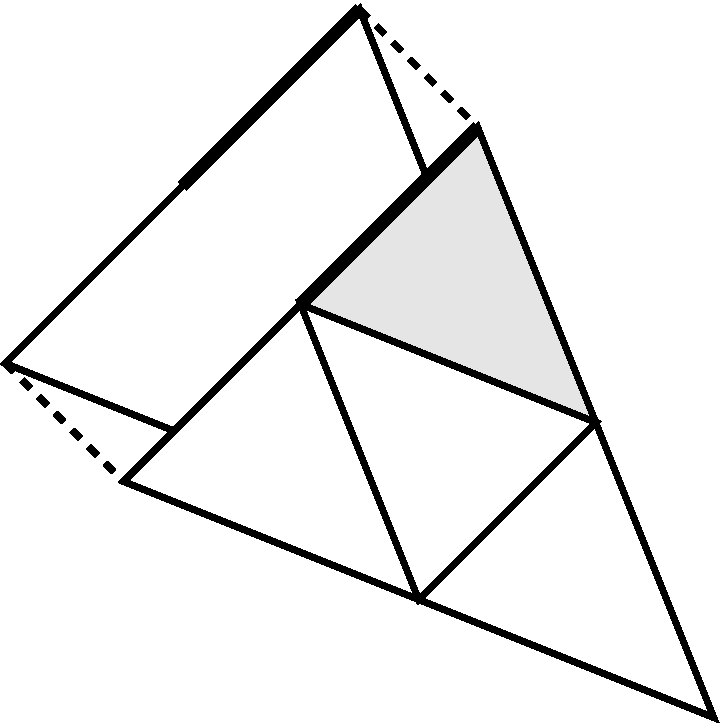
\includegraphics[width=.5\textwidth]{figs/adaptive}
    \end{center}
  \end{figure}
\end{minipage}
\begin{minipage}[h]{.45\textwidth}
\begin{eqnarray*}
u^F & = & u^C \\
\sum_i u_i^F \phi_i^F & = & \sum_j u_j^C \phi_j^C \\
A_{ki} u_i & = & B_{kj} u_j \\
u_i & = & A_{ki}^{-1} B_{kj} u_j
\end{eqnarray*}
\end{minipage}

Integrated values (and fluxes, for $C^1$ continuity) give
element-independent matrices:
\begin{eqnarray*}
A_{ki} & \equiv & (\phi_i^F, \phi_k^F) \\
B_{kj} & \equiv & (\phi_j^C, \phi_k^F)
\end{eqnarray*}

}


%%%%%%%%%%%%%%%%%%%%%%%%%%%%%%%%%%%%%%%%%%%%%%%%%%%%%%%%%%%%%%%%%%%%%
\royslide{Adaptive $p$ Constraints}{

\begin{minipage}[h]{.45\textwidth}
\begin{center}
\includegraphics[width=.9\textwidth]{figs/PHierarchic}
\end{center}
\end{minipage}
\begin{minipage}[h]{.45\textwidth}
\royitemizebegin
\item $p$ refinement is well suited to hierarchic adaptivity
\item Hanging degree of freedom coefficients are simply set to 0
\royitemizeend
\end{minipage}
}


%%%%%%%%%%%%%%%%%%%%%%%%%%%%%%%%%%%%%%%%%%%%%%%%%%%%%%%%%%%%%%%%%%%%%
\royslide{Error Indicators}{

Integration by parts gives an upper error bound on subelements $S$ for
the biharmonic problem:

\begin{eqnarray*}
   \norm{e}_{H^2(\Omega)} & \leq & C_\Omega
   \sum_S \left[\norm{f - \Delta^2 u_h}_S h_S^{2} + \right. \\
& & \left.
   \frac{1}{2} \norm{\jump{\dn{\Delta u_h}}}_{\partial S} h_S^{3/2} +
   \frac{1}{2} \norm{\jump{\Delta u_h}}_{\partial S} h_S^{1/2} \right]
\end{eqnarray*}

The most significant term gives a simple indicator on elements $K$ for
more general fourth order problems:

\[ \eta_K \equiv \sqrt{h_K} \norm{\jump{\Delta u_h}}_{\partial K}
\]

}



%%%%%%%%%%%%%%%%%%%%%%%%%%%%%%%%%%%%%%%%%%%%%%%%%%%%%%%%%%%%%%%%%%%%%
\royslide{Diffuse Interface Modeling with AMR/C}{

\begin{minipage}[h]{.45\textwidth}
\begin{center}
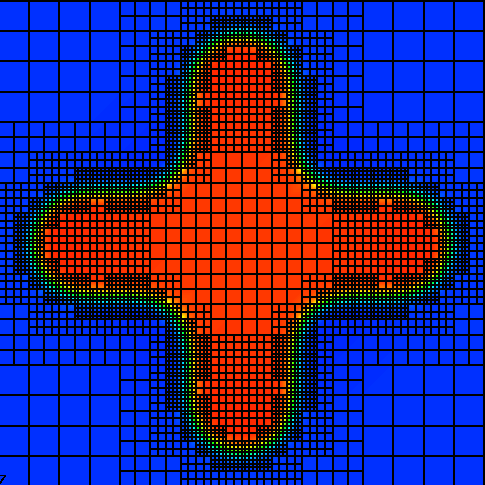
\includegraphics[width=.9\textwidth]{figs/cross-adaptive}
\end{center}
\end{minipage}
\begin{minipage}[h]{.45\textwidth}
\royitemizebegin
\item Mesh coarsening in smooth regions is traded for mesh
refinement in sharp layers
\item Equivalent accuracy is achieved here with 75\% fewer degrees of
freedom than a uniform mesh
\royitemizeend
\end{minipage}

}



%%%%%%%%%%%%%%%%%%%%%%%%%%%%%%%%%%%%%%%%%%%%%%%%%%%%%%%%%%%%%%%%%%%%%
\royslide{Diffuse Interface Modeling with AMR/C}{

\begin{minipage}[h]{.45\textwidth}
\begin{center}
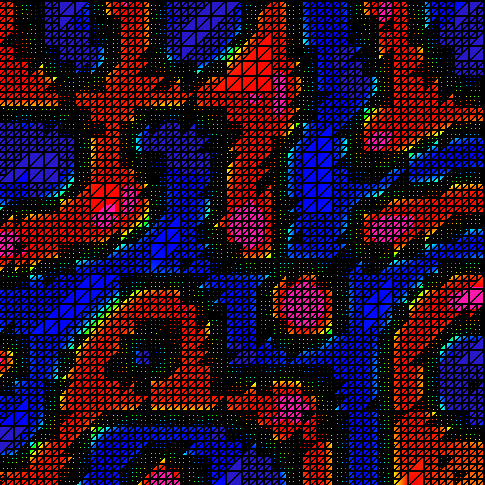
\includegraphics[width=.9\textwidth]{figs/spinodal-adaptive}
\end{center}
\end{minipage}
\begin{minipage}[h]{.45\textwidth}
\royitemizebegin
\item Adaptive Mesh Refinement / Coarsening reduces solver expense
\item Laplacian Jump error indicator tracks moving interfaces
\royitemizeend
\end{minipage}

}



%%%%%%%%%%%%%%%%%%%%%%%%%%%%%%%%%%%%%%%%%%%%%%%%%%%%%%%%%%%%%%%%%%%%%
\royslide{Adaptive Refinement Strategies}{

Maintaining a constant global error estimate:
\royitemizebegin
\item Tracks time-varying complexity
\item Gives reliable results
\item Requires reliable error bounds
\royitemizeend

Maintaining constant element count:
\royitemizebegin
\item Keeps an upper bound on computational expense
\item Only requires a good feature indicator
\royitemizeend

}
